% background.tex:

\chapter{BACKGROUND} % all caps please
\label{chap:background}



%%% Section
\section{Basics of Optical Imaging}
\label{chap:background:basics}

\subsection{Light-Tissue Interactions}
Biological optical imaging has the capability to detect biological structure, function, and molecular characteristics based on photon interactions with tissue~\cite{Wang2009}. The interaction of light with tissue is governed primarily by three processes: reflection, scattering, and absorption~\cite{Welch2010}.

\begin{figure}
    \begin{center}
    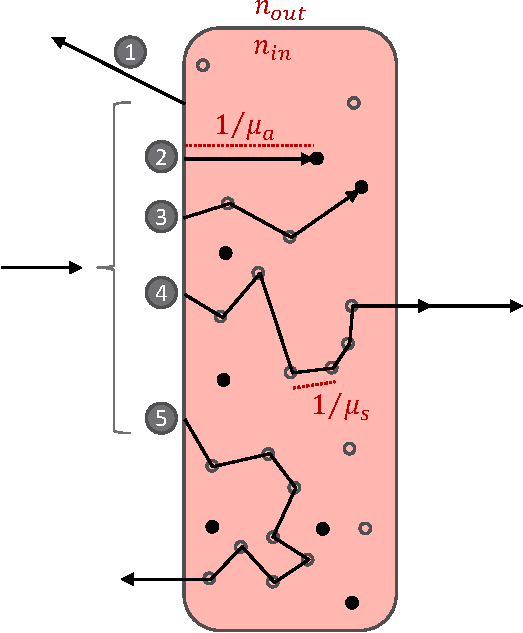
\includegraphics[width=.35\textwidth]{fig/background/lightinteraction.pdf}
    \end{center}
    \caption{Possible interactions when light interfaces with tissue. The pink rectangle represents tissue. White circles are scatterers. Black dots are absorbers.  (1) Light reflects without entering the tissue. (2) Light immediately gets absorbed. (3) Light scatters multiple times before being absorbed. (4) Light scatters multiple times before exiting the tissue on the opposite side it entered. (5) Light scatters multiple times but exits on the side it entered. } 
    \label{fig:lightinteraction}
\end{figure} 

The index of refraction, $n$, is a unitless number that describes how fast light travels through material~\cite{Wang2009}. It is used to determine how much the path of light is bent upon transitioning from one material to the next.  This is governed by Snell’s Law of Refraction~\cite{Wang2009}, $n_1 \times sin\theta_1= n_2\times sin\theta_2$, which define the angle of incidence, $\theta_1$, and angle of refraction, $\theta_2$, based on two media with indices of refraction $n_1$ and $n_2$. Thus, from Snell’s Law, we can also determine the amount of light that is reflected when reaching an interface (Figure~\ref{fig:lightinteraction}). 

Once photons enter a turbid media, they move in all directions and may be scattered or absorbed (Figure~\ref{fig:lightinteraction}). Absorption depends on the component concentrations of tissue~\cite{Nunez2018}. In the visible to near-infrared wavelength range, the primary absorption components include water, hemoglobin, pigment, and lipid~\cite{Du2006, Pogue2006}. The absorption coefficient, $\mu_a$ [$cm^{-1}$], is defined such that, when a photon propagates over an infinitesimal distance $ds$, the probability of absorption is $\mu_a\times ds$~\cite{Welch2010}. The absorption coefficient depends on the molar extinction coefficient of a given chromophore $\epsilon$ [$cm^{-1}\times M^{-1}$], and its Molar concentration, $c$. Thus, the absorption coefficient per wavelength is 

\begin{equation}
    \mu_a(\lambda) = log(10) \sum_{i=1}^{t}\epsilon_i(\lambda)\times c_i~\cite{Nunez2018}. 
\end{equation}
where t is the total number of absorbing components in the tissue. From this, we deduce that $1/\mu_a$ is the average path length traveled by a photon before being absorbed. 

Light entering a tissue can also undergo scattering events, events during which directionality changes occur due to biological structures within the media (Figure~\ref{fig:lightinteraction}). In the visible to infrared wavelength range, the primary scattering components in biological tissue are protein, fat, and mitochondria~\cite{Du2006, Pogue2006}. Analogously, the scattering coefficient, $\mu_s$, is defined such that, when a photon propagates over an infinitesimal distance $ds$, the probability of scattering is $\mu_s\times ds$~\cite{Welch2010}. Additionally, we model the probability distribution of scattered photons by an angular function known as the anisotropy factor, $g$~\cite{Wang2009}. Since $g$ is based on the scattering angle, the closer to 1.0 $g$ is, the more likely the photon is to be scattered in the forward direction. To account for this anisotropy factor, we define the reduced scattering coefficient, $\mu_s^{'}$, as 
$\mu_s^{'} = \mu_s(1-g)$~\cite{Wang2009}. The average distance traveled by a photon between scattering events is $1/\mu_s$.


\subsection{Components of Optical Measurement Systems}
Optical systems are composed of three elementary blocks: a source that radiates light, a sample through which light propagates, and a detector that measures the light intensity after photons have traveled through the sample~\cite{Webster2010}. Although there are numerous types of sources and detectors, here, we highlight only the types used in the optical systems developed for this thesis. 

\ac{LED} are devices that radiate light when a current passes through them~\cite{Webster2010}. They are ubiquitous in modern electronics due to being inexpensive and requiring minimal power to operate. In our \ac{MOXI} system, we leverage the white LEDs used for flash photography common in most smartphones. Our \ac{MOBI} system uses dual-wavelength \ac{LED}s chosen to optimize propagation within the brain layers. Arrays of \ac{LED}s are used in conjunction with digital micromirrors to project color images from projectors. Our \ac{OMCI} system uses an \ac{LED} projector to shine patterns to scan the surface of the breast. For certain applications, it is better to have a light source that does not spread out much, such as \ac{LASER}. Laser light sources produce very narrow beams of light. In \ac{OMCI}, we use a laser to input light into a projector to project patterns onto the breast. 

Detectors are devices used to measure light. Photodiodes are the reverse of \ac{LED}s\textemdash they convert light into electrical current~\cite{Webster2010}. Their cost tends to be relative to their sensitivity. \ac{MOXI} and \ac{MOBI} use inexpensive photodiodes chosen to be sensitive to the wavelengths of their associated \ac{LED}s. \ac{OMCI} uses cameras to detect the reflection and transmission of projected patterns. These cameras capture light through a small lens using a tiny array of microscopic detectors. 

The measured light, in combination with the known type of source, allows for the determination of biological structure, function, and molecular characteristics of the tissue through which the light propagated. For example, the detection of photons from particular wavelengths allows us to compute concentrations of oxygenated ($HbO_2$) and de-oxygenated ($HbR$) hemoglobin in tissue. From this, we can infer parameters such as total hemoglobin concentration and tissue oxygen saturation~\cite{Nunez2018}. 
%From this, we can infer parameters such as total hemoglobin concentration (THC=HbR+HbO_2) and tissue oxygen saturation (S〖tO〗_2=  (HbO_2)⁄((HbR+ HbO_2)))[3]. 


\subsection{Optical Phantom Fabrication}
Phantoms are objects with optical properties that mimic human tissues~\cite{Pogue2006}. They are common for evaluating the performance of \ac{NIR} imaging systems~\cite{Pogue2006}. To mimic \ac{NIR} light propagation due to components within biological tissue, phantoms typically attempt to mimic the reduced scattering coefficient ($\mu_s^{'}$) and the wavelength-dependent absorption coefficient ($\mu_a$) in biological tissue~\cite{Dempsey2017}. Traditionally, these phantoms are created using recipes that involve a mix of scattering agents and absorbing pigments with a base~\cite{Hebden1995,Dong2015}. The geometry of the phantom is typically created using either mold casting~\cite{Hahn2012,Mobashsher2014} or spin coating~\cite{Park2013}. While useful for simple phantoms, these methods fall short in supporting complex geometries needed for phantoms requiring structural and physiological properties, such as when \ac{DOT} is used to image the brain~\cite{Hebden2002,Villringer1997}. Thus, a new method to manufacture phantoms with spatially varying optical properties and anatomically accurate geometries is needed to support the system development, calibration, and testing of new imaging protocols~\cite{Cerussi2012,Diep2015}.  



%%% Section
\section{Imaging Techniques}
\label{chap:background:techniques}
\subsection{Pulse Oximetry}
Pulse oximetry is used to measure oxygen saturation of hemoglobin in arterial blood and is so widely prevalent it is regarded as the fifth vital sign in medical care~\cite{Neff1988}. It is based on two principles. The first is that $HbO_2$ and $HbR$ absorb red and \ac{IR} light differently~\cite{Bohn2015}. Because of this, pulse oximeters tend to emit two wavelengths of light. Traditional (finger-clip) pulse oximeters place light sources and detectors on opposite sides of the finger. The second principle is that arterial blood volume fluctuates with the cardiac cycle while blood volume in veins, capillaries, skin, fat, and bone remains relatively constant~\cite{Sinex1999}. Thus, light that propagates through the finger and is detected by the detector has two components during temporal measurements of the cardiac cycle\textemdash a relatively stable and non-pulsatile \ac{DC} component from the constant volume in veins and capillaries, and a pulsatile \ac{AC} component from the volume fluctuation of the arteries~\cite{Lopez2012}. This detected time trace is called a \ac{PPG}~\cite{Sinex1999}. 

Pulse oximeters use the amplitudes of \ac{PPG} signals from red and \ac{IR} light to calculate oxygen saturation ($SpO_2$) at the finger. $SpO_2$ is calculated from the ratio of the \ac{AC} to \ac{DC} components of the red and \ac{IR} light. The \ac{RR} is defined as
\begin{equation} \label{eq:RR}
    RR = \frac{ A_{red,AC}/A_{red,DC} }{ A_{IR,AC}/A_{IR,DC} }
    %RR = \frac{\frac{A_{red,AC}}{A_{red,DC}}}{\frac{A_{IR,AC}}{A_{IR,DC}}} 
\end{equation}
where $A$ is absorbance. At low oxygen saturation, the increased $HbR$ presence leads to a larger relative change in amplitude of red light due to the pulse compared to \ac{IR} absorbance ($A_{red,AC} > A_{IR,AC}$), resulting in a higher $RR$ value. $SpO_2$ is calculated from a calibration curve mapping $RR$ to $SpO_2$ generated from empirical measurements of $RR$ in healthy volunteers with altered saturations~\cite{Chan2013}. 


\subsection{Functional Near-Infrared Spectroscopy}
\Ac{fNIRS} is an emerging neuroimaging technique that uses low-power near-infrared light to measure hemodynamic changes due to brain activities~\cite{Boas2014}. It is based on three fundamental principles. The first is that human tissue is relatively transparent to light in the near-infrared range allowing photons to propagate~\cite{Ferrari2012}. Secondly, hemoglobin has unique absorbing characteristics that allow for oxygenation-dependent quantification of \ac{NIR} light absorption~\cite{Ferrari2012}. The third is the theory of neurovascular coupling, which states that the brain’s demand for oxygen is altered by neuronal activation. fNIRS assumes that changes in hemoglobin concentrations are indicators of brain activity~\cite{Boas2014}. 

In \ac{fNIRS}, multiple sources and detectors are placed on the scalp over a \ac{ROI}~\cite{Scholkmann2014}. The photons travel through the head being scattered and absorbed by the different tissue types~\cite{Pinti2020} (scalp, skull, cerebrospinal fluid, and neuronal tissue) until the non-absorbed components of the scattered light are detected by a detector~\cite{Bunce2006,Izzetoglu2007}. The activity-dependent local increase of $HbO$ and decrease of $HbR$ change the absorption rate of neuronal tissue and affect the intensity of light detected~\cite{Izzetoglu2007, Perrey2008}. This change in intensity, along with the absorption spectra of chromophores, allows for the calculation of $HbO$ and $HbR$ concentrations via the modified Beer-Lambert law~\cite{Scholkmann2014}. 


\subsection{Diffuse Optical Tomography}
\ac{DOT} is a non-invasive imaging technique for 3-D functional tissue characterization~\cite{Boas2001}. This is done through the illumination of tissue with an array of light sources and the measurement of the exiting light with an array of detectors~\cite{Culver2001}. Typically, a source in the array is turned on and the light is measured by all detectors for that source. This is repeated sequentially for each source. A model of light propagation from the source to detector locations is parameterized using unknown scattering and absorption coefficients of the illuminated tissue~\cite{Arridge1999}. The propagation model is then ``inverted'' to determine the scattering and absorption parameters of the tissue~\cite{Arridge1999}. The inversion of the model is the solution to the question ``given my array of sources, what optical parameters must my tissue possess in order to produce the results I measured with my array of detectors?''

Although conceptually simple, in practice, \ac{DOT} is plagued with difficulties. The use of diffusive light along with the inherent ill-posedness of the inverse reconstruction leads to low spatial resolution results~\cite{Arridge2009, Durduran2010}. Additionally, the sensitivity to tissue-optode coupling coefficients of the course spatial sampling leads to an inaccurate representation of tissue properties~\cite{Schweiger2007}. To address low spatial resolution, the use of tissue structural priors (structural data obtained from MRI~\cite{Pearlman2012}, ultrasounds~\cite{Zhu2010}, or x-ray~\cite{Fang2011, Deng2015}) have been recently used to better constrains the inverse problem and produced higher resolution images~\cite{Pearlman2012}. Wide-field illumination (the projection of a pattern image rather than a few spare source points) and camera-based detection (where a pixel in a camera acts as a detector in an array) has allowed for high-density sampling and acceleration of data acquisition~\cite{Belanger2010}. 


\subsection{Structured-Light Imaging}
One method of improving \ac{DOT} reconstructions is to further constrain the inverse problem through highly accurate breast surface estimations. However, the two most prominent techniques for 3-D breast surface imaging (stereophotogrammetry and laser scanning~\cite{Yang2015}), require a large number of cameras and precise installation, making them infeasible in the confined, low-light mammography setting. An emerging, non-invasive 3-D surface imaging technique is \ac{SLI}. \ac{SLI} works by illuminating an object with 2-D spatially varying patterns and using an imaging sensor (e.g. a camera) to capture the illuminated object~\cite{Geng2011}. The distortion of the specially designed patterns inform of the geometric properties of the object. Calibration of the projector-camera system is easily done by capturing images of a known planar pattern~\cite{Moreno2012a}. With the ability to use off-the-shelf components, its use with a single projector and camera, and a robust and simple calibration method, SLI is positioned to be an accurate, fast, and cost-effective breast surface imaging system.



%%% Section
\section{``-ilities'' of Near-infrared Imaging Systems}
\label{chap:background:ilities}
In general, medical instruments can be approached from multiple viewpoints~\cite{Webster2010}. They can be classified according to clinical medicine specialties (pediatrics, cardiology, radiology, etc.), the principle of transduction (ultrasonic, electrochemical, capacitive, etc.), or they can be studied separately for each organ system (pulmonary, nervous, endocrine, etc.)~\cite{Bushberg2011}. In this thesis, we focus on optical imaging in the near-infrared range. These systems can be classified as a radiology specialty with the principle of transduction being optical measurements perturbed by hemodynamics. We intentionally have not chosen a particular organ system to focus on so as not to limit the potential application of optical imaging. 

We will compare the three \ac{NIR} imaging systems in terms of their system lifecycle properties, or ilities~\cite{DeWeck2012}. While it is true that any system has a set of design criteria based on signal, environmental, medical, and economic factors that impose constraints based on their specific use, ilities are typically not primary functional requirements of a system. Rather, ilities often manifest themselves after a system has been put to initial use. Unlike other engineering properties that are more easily tested in a laboratory, ilities tend to not receive as much focus~\cite{DeWeck2012}. However, when discussing the potential translation of a medical technology to outside the laboratory setting, ilities better inform of wider system impact with respect to stakeholders and are better indicators of user needs~\cite{DeWeck2011}. The ilities we will use in this thesis to compare across the three \ac{NIR} systems are defined in Table~\ref{tab:ilities}. 

\begin{table}
\centering
\caption{Definition of ilities. Asterisks indicate the definition was replicated from de Weck et al., 2012~\cite{DeWeck2012}}
\label{tab:ilities}
\resizebox{\textwidth}{!}{%
\begin{tabular}{@{}ll@{}}
\toprule
Ility Name         & Definition (``ability of a system...'')                                                                   \\ \midrule
Adaptability*      & to be used for other applications besides what it was designed for with an acceptable level or resource \\
Affordability      & to be purchased with minimal investment                                                                 \\
Comfortability     & to be used extensively while actively measuring                                                         \\
Conformability     & to physically match the surface it is trying to measure                                                 \\
Extensibility*     & to accommodate new features after design                                                                \\
Interoperability*  & to effectively interact with other systems                                                              \\
Maintainability    & to remain in working condition with minimal or no component replacement                                 \\
Manufacturability  & to be built using minimal components and fabrication methods                                            \\
Modifiability*     & to change the current set of specified system parameters                                                \\
Operability        & to be operated by a non-technical user                                                                  \\
Portability        & to be transported to another location with minimal resources                                            \\
Reconfigurability* & to change its component arrangement and links reversibly                                                \\ \bottomrule
\end{tabular}%
}
\end{table}



% --- EOF ---